% To je predloga za poročila o domačih nalogah pri predmetih, katerih
% nosilec je Blaž Zupan. Seveda lahko tudi dodaš kakšen nov, zanimiv
% in uporaben element, ki ga v tej predlogi (še) ni. Več o LaTeX-u izveš na
% spletu, na primer na http://tobi.oetiker.ch/lshort/lshort.pdf.
%
% To predlogo lahko spremeniš v PDF dokument s pomočjo programa
% pdflatex, ki je del standardne instalacije LaTeX programov.

\documentclass[a4paper,11pt]{article}
\usepackage{a4wide}
\usepackage{fullpage}
\usepackage[utf8x]{inputenc}
\usepackage[slovene]{babel}
\selectlanguage{slovene}
\usepackage[toc,page]{appendix}
\usepackage[pdftex]{graphicx} % za slike
\usepackage{setspace}
\usepackage{color}
\definecolor{light-gray}{gray}{0.95}
\usepackage{listings} % za vključevanje kode
\usepackage{hyperref}
\renewcommand{\baselinestretch}{1.2} % za boljšo berljivost večji razmak
\renewcommand{\appendixpagename}{Priloge}

\lstset{ % nastavitve za izpis kode, sem lahko tudi kaj dodaš/spremeniš
language=Python,
basicstyle=\footnotesize,
basicstyle=\ttfamily\footnotesize\setstretch{1},
backgroundcolor=\color{light-gray},
}

\title{Linearna regresija}
\author{Gregor Majcen (63070199)}
\date{\today}

\begin{document}

\maketitle

\section{Uvod}
Peta domača naloga je namenjena izdelavi različnih algoritmov za linearno regresijo. Vsak algoritem je dober na t.i. domačem terenu in naš cilj je te algoritme implementirati in primerjati. Podatki, s katerimi primerjamo te algoritme so poljubni, pogoj je le, da so zvezni.

\section{Podatki}
Za podatke sem vzel že narejeno tabelo “housing'', ki je na voljo tudi v Orange. To tabelo sem izbral zato, ker sem jo našel uporabljeno v Orange dokumentaciji za linearno regresijo in sem lahko primerjal tudi rezultate Orange algoritma. Zaradi lepših grafov sem vse vrednosti v tabeli delil s 3.

Tabela vsebuje 14 atributov, 506 primerov in ne vsebuje praznih vrednosti. Atributi so realna števila, ravno tako razred.

\section{Rezultati}

\subsection{Grafičen prikaz izbranega atributa}
Izmed štirinajstih atributov sem si izbral sedmega, razlog pa je en sam: najlepše porazdeljene točke.

Na slikah od~\ref{fig:figure1} do~\ref{fig:figure2} je razvidna razlika med različnima natančnostima, ki je določen z mejo $\varepsilon$. Manjši kot je $\varepsilon$, boljši so rezultati, saj algoritem deluje toliko časa, da je absolutna vsota vseh razlik prejšnjih in sedanjih izračunanih $\theta$ manjša kot $\varepsilon$. Lahko bi temu tudi rekli do konvergiranja, ampak z določenim odstopanjem $\varepsilon$. Na sliki~\ref{fig:figure1} imamo $\varepsilon$ enak $10^{-3}$ in je rezultat najden v 378 korakih (izračunov $\theta$). Če pa $\varepsilon$ nastavimo na $10^{-5}$ pa potrebujemo 917 korakov, ampak dobimo vidno boljši rezultat. Velikost koraka ($\alpha$) sem nastavil na največji možen, da še zmerom konvergira, to je 0.0001. To je mogoče doseči le s testiranjem, saj če je $\alpha$ prevelik J ocena nikoli ne doseže pričakovanega minimuma, saj se zaradi prevelikega koraka odbije in napaka posledično le narašča.

V levem stolpcu slik so prikazane J ocene, ter z črnimi “x'' pot, ki je narejena z določeno metodo. Rdeča pika pomeni ciljno točko, črn velik križ pa točko, ki je dosežena z analitično metodo. Tako je lepo razvidna napaka. Čeprav napaka izgleda majhna, je v desnem stolpcu slik videti večja. Zelena črta prikazuje izračunano metodo, rdeča pa analitično metodo. 

Iz slik je razvidno tudi, da sta si paketna in stohastična metoda zelo podobni, vendar se pri vseh atributih izkaže drugače, kot je prikazano na tabeli~\ref{t:rez}.

\begin{figure}[h!]
\begin{minipage}[b]{0.5\linewidth}
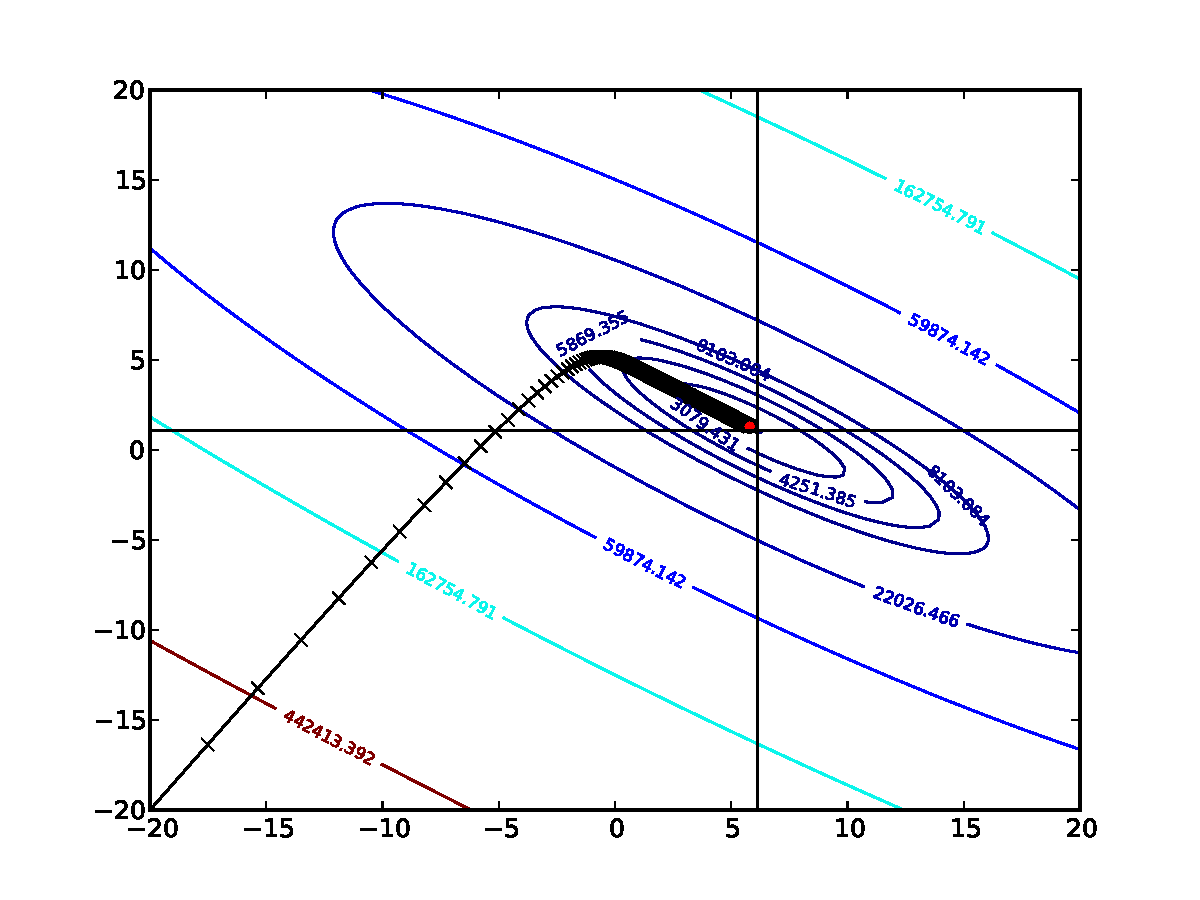
\includegraphics[scale=0.4]{n31.pdf}
\caption{Stohastična metoda z $\varepsilon$=$10^{-3}$}
\label{fig:figure1}
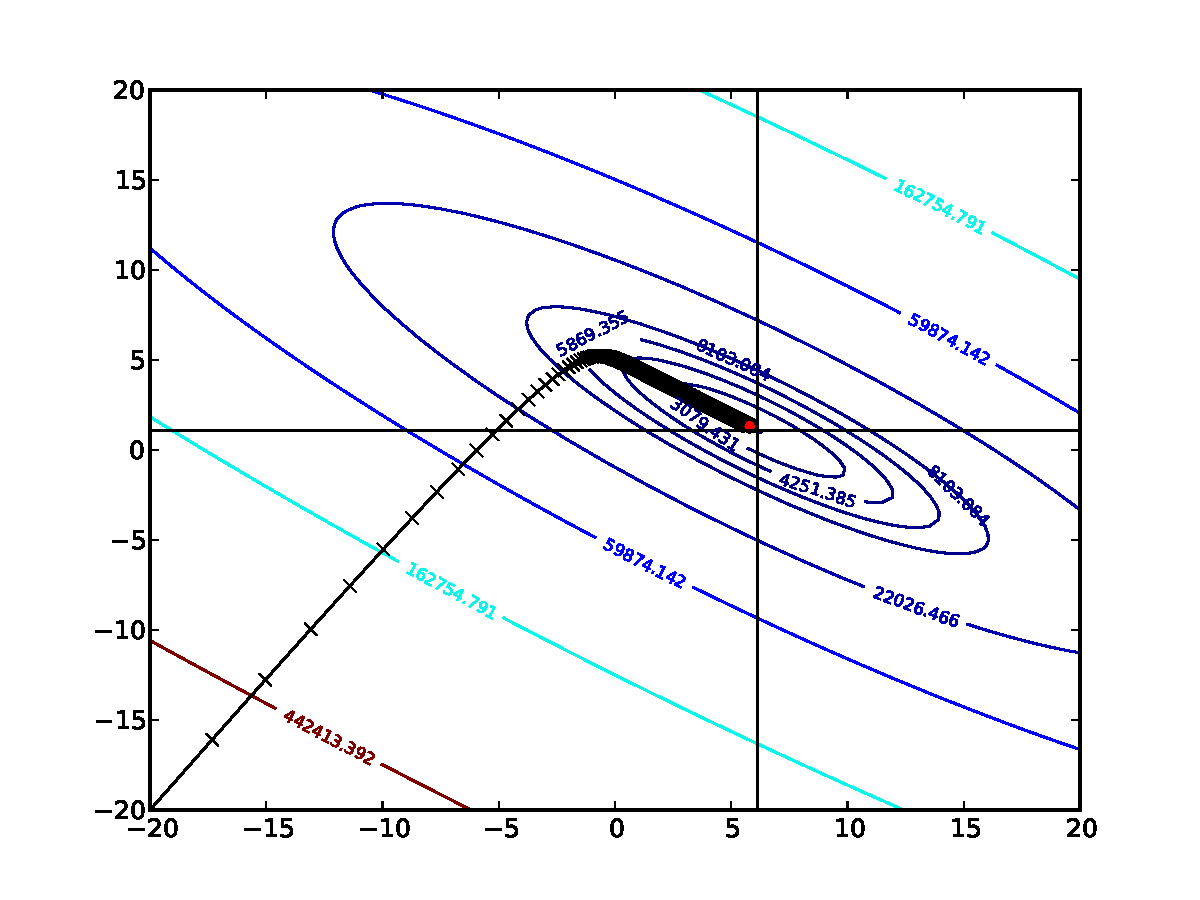
\includegraphics[scale=0.4]{b31.pdf}
\caption{Paketna metoda z $\varepsilon$=$10^{-3}$}
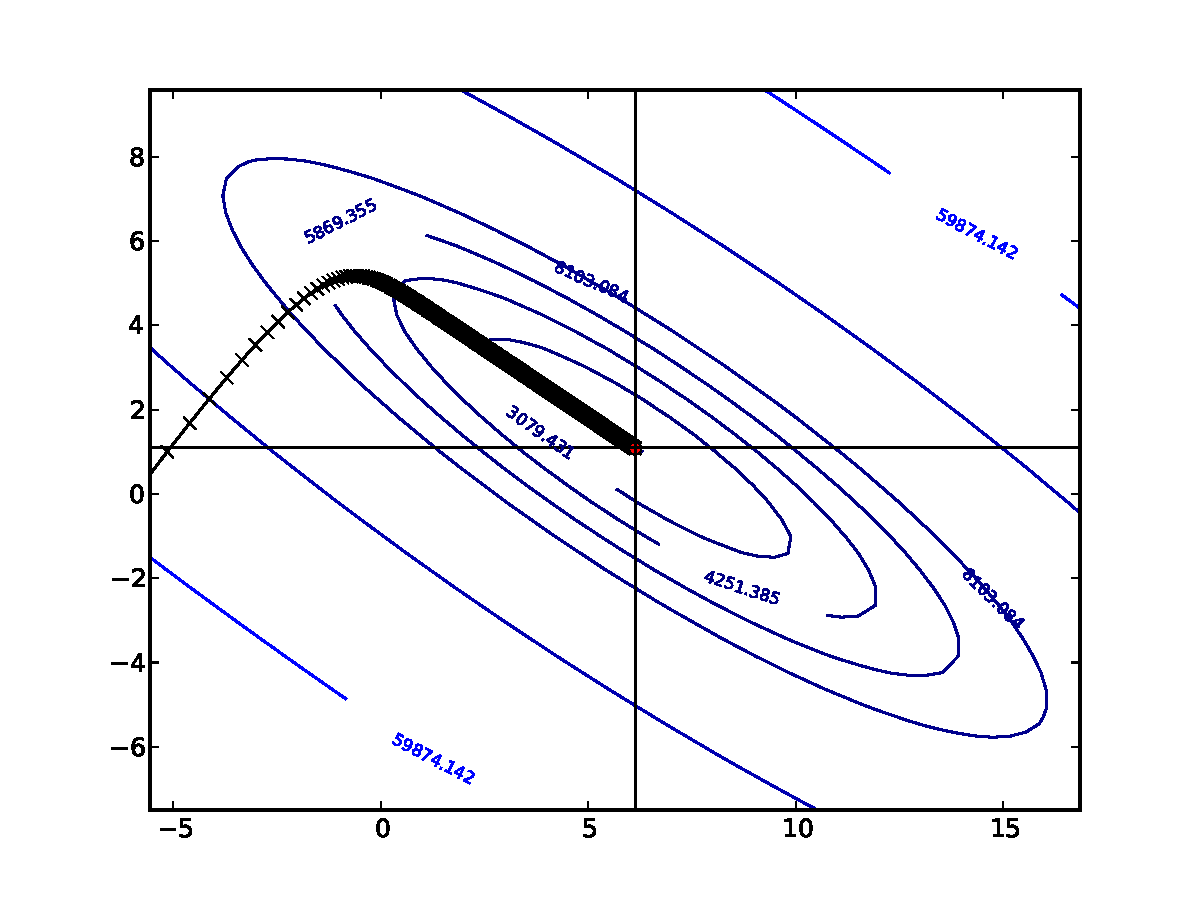
\includegraphics[scale=0.4]{b51.pdf}
\caption{Obe metodi z $\varepsilon$=$10^{-5}$}
\end{minipage}
\hspace{0.5cm}
\begin{minipage}[b]{0.5\linewidth}
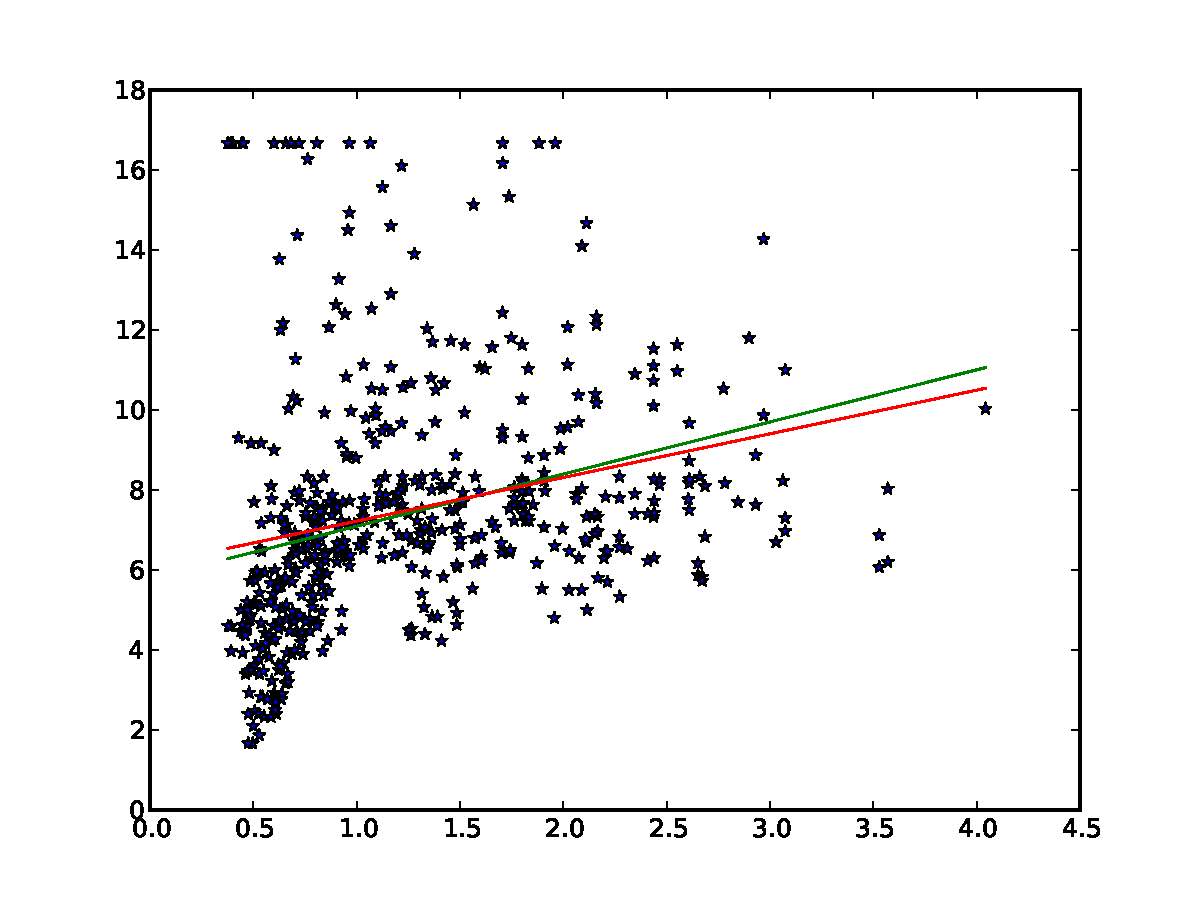
\includegraphics[scale=0.4]{n32.pdf}
\caption{Stohastična metoda z $\varepsilon$=$10^{-3}$}
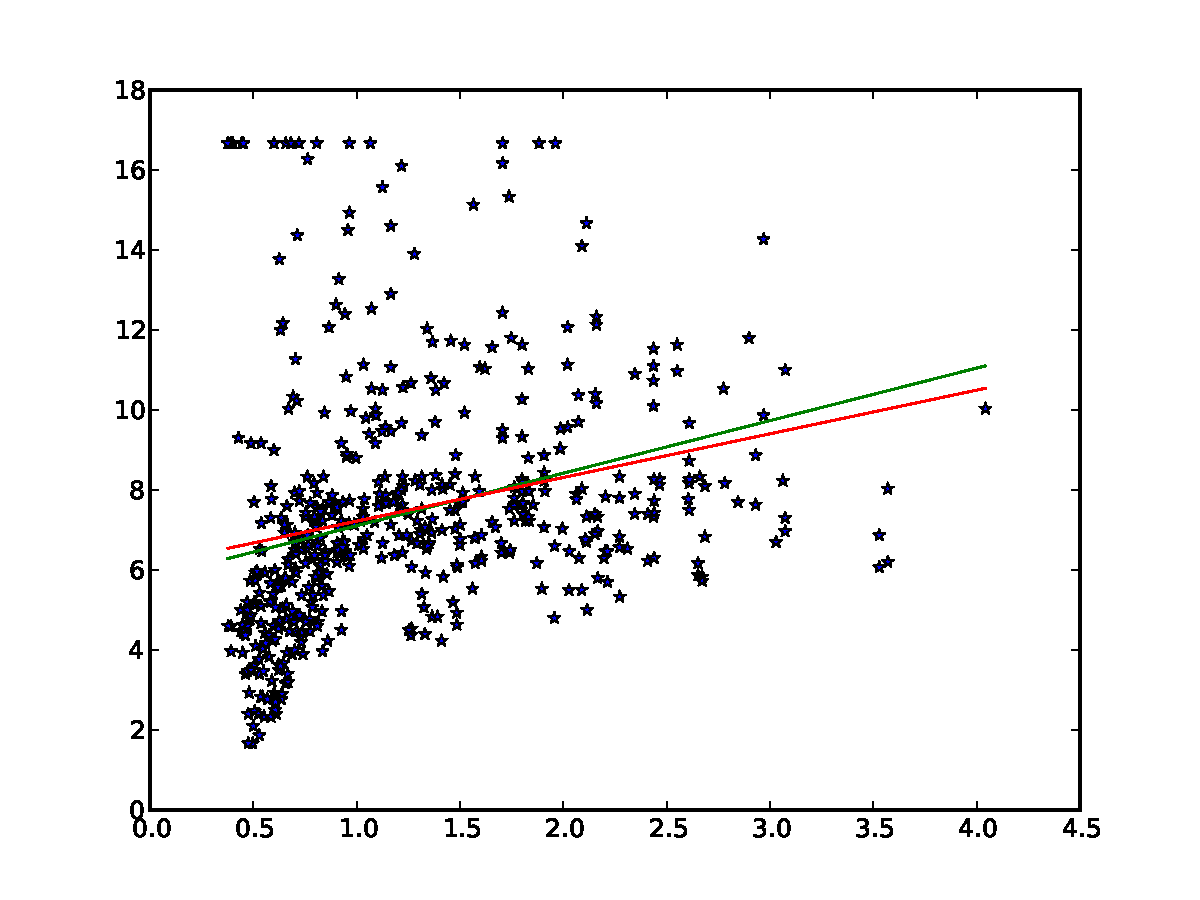
\includegraphics[scale=0.4]{b32.pdf}
\caption{Paketna metoda z $\varepsilon$=$10^{-3}$}
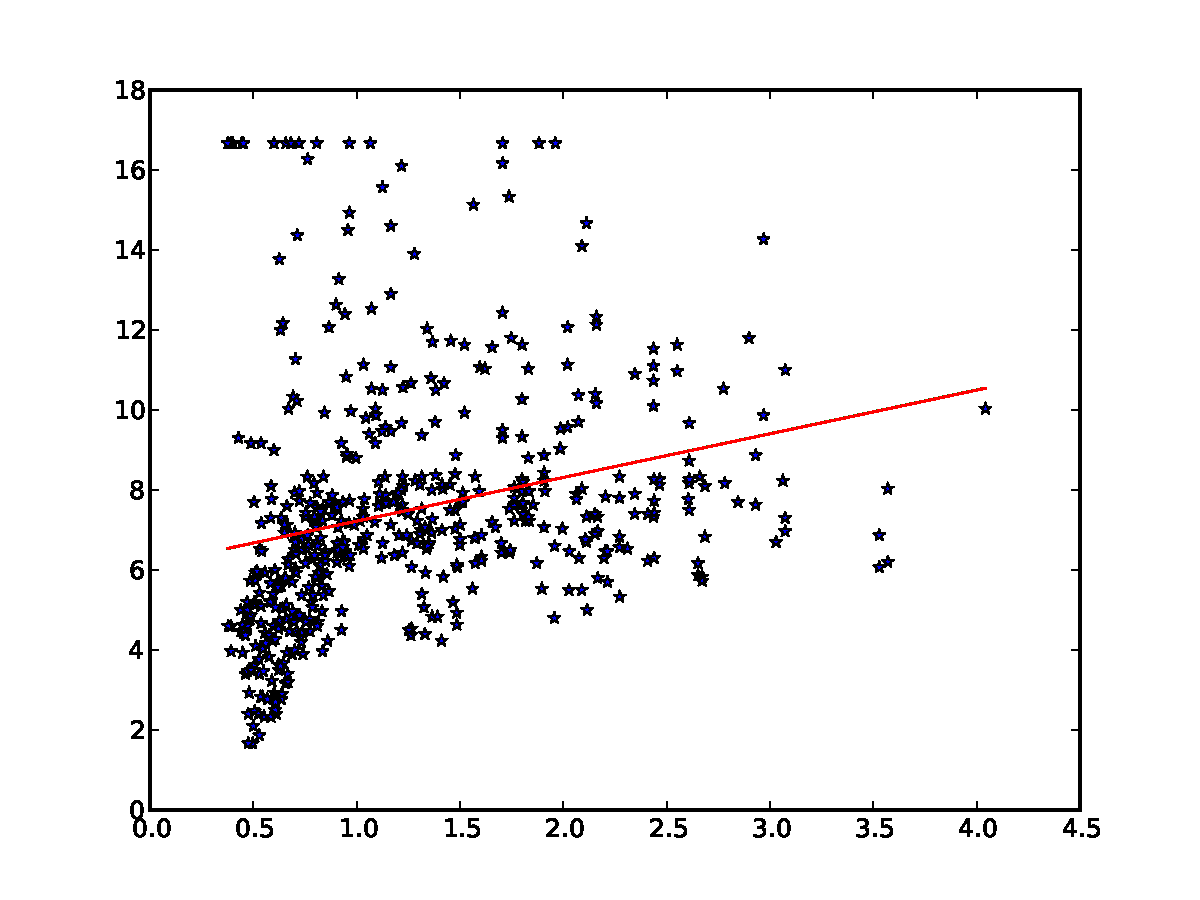
\includegraphics[scale=0.4]{b52.pdf}
\caption{Obe metodi z $\varepsilon$=$10^{-5}$}
\label{fig:figure2}
\end{minipage}
\end{figure}

\subsection{Rezultati vseh atributov}
Pri obeh metodah sem uporabljal $\varepsilon$ mejo $10^{-5}$. Za primerjavo sem uporabil oceno J.

$J(\theta) = {1\over2} \sum_{i=1}^m ((\theta^Tx^{(i)}) - y^{(i)})^2$

V tabeli~\ref{t:rez} so zapisani rezultati celotne housing tabele za stohastično metodo (SM): J=733, 1001628 iteracij, paketno metodo (BM): J=1635, 940849 iteracij in analitično (AM): J=615. J ocena nam pove kvadratno napako med pravilnim in izračunanim rezultatom. Za naš primer opazimo, da je najbolj primerna analitična metoda, ampak zaradi množenja matrik, ki je $O(n^3)$, lahko pri zelo veliki količini podatkov porabi preveč časa. Če pa izbiramo le med stohastično in paketno, se je pa stohastična izkazala za boljšo. 

\begin{table}[h]
\centering
\begin{tabular}{l|l|l|l}
$\theta$ & SM & BM & AM \\
\hline
0 & 3.40771294 & -8.65614691 & 10.21531638\\
1 & -0.135737901 & -0.119746420 & -0.108011354\\
2 & 0.0357196662 & 0.0568844863 & 0.0464204559\\
3 & 0.0891750653 & 0.250145010 & 0.0205586763\\
4 & 0.755742642 & -10.28511096 & 2.68673389\\
5 & -13.8276397 & -10.78191477 & -10.77666148\\
6 & 5.31945778 & 8.72749238 & 3.80986498\\
7 & 0.00785609675 & 0.0397324835 & 0.000692223854\\
8 & -1.05219413 & -0.762339775 & -1.47556679\\
9 & 0.136973014 & 0.184630329 & 0.306049515\\
10 & -0.00759340766 & -0.00996154857 & -0.0123345932\\
11 & -0.441920824 & -0.0796754944 & -0.952747256\\
12 & 0.00957698475 & 0.0250695631 & 0.00931168341\\
13 & -0.465608380 & -0.296737765 & -0.524758397\\
\end{tabular}
\caption{tabela rezultatov}
\label{t:rez}
\end{table}

\section{Izjava o izdelavi domače naloge}
Domačo nalogo in pripadajoče programe sem izdelal sam.

\end{document}
